% Figure: 17x17 confusion matrix, ConvNeXt-Tiny, counts summed over 3 seeds
% Source     : docs/reports/experiments/phase_1b/final_b_new_recomputed/
%              20260819T043733Z/predictions.csv   (only source of the counts)
% Cross-check: confusion_matrices.npz, exact element-wise after permuting to
%              the family class order -- 0 cells differing on all three seeds
% Artifacts  : artifact/person3/confusion/{confusion_convnext_main.csv,
%              confusion_convnext_main_per_seed.csv, confusion_metadata.json}
% Run ids    : taskB17__main__seed_{42,123,456}__convnext_tiny
\begin{figure}[!htbp]
\centering
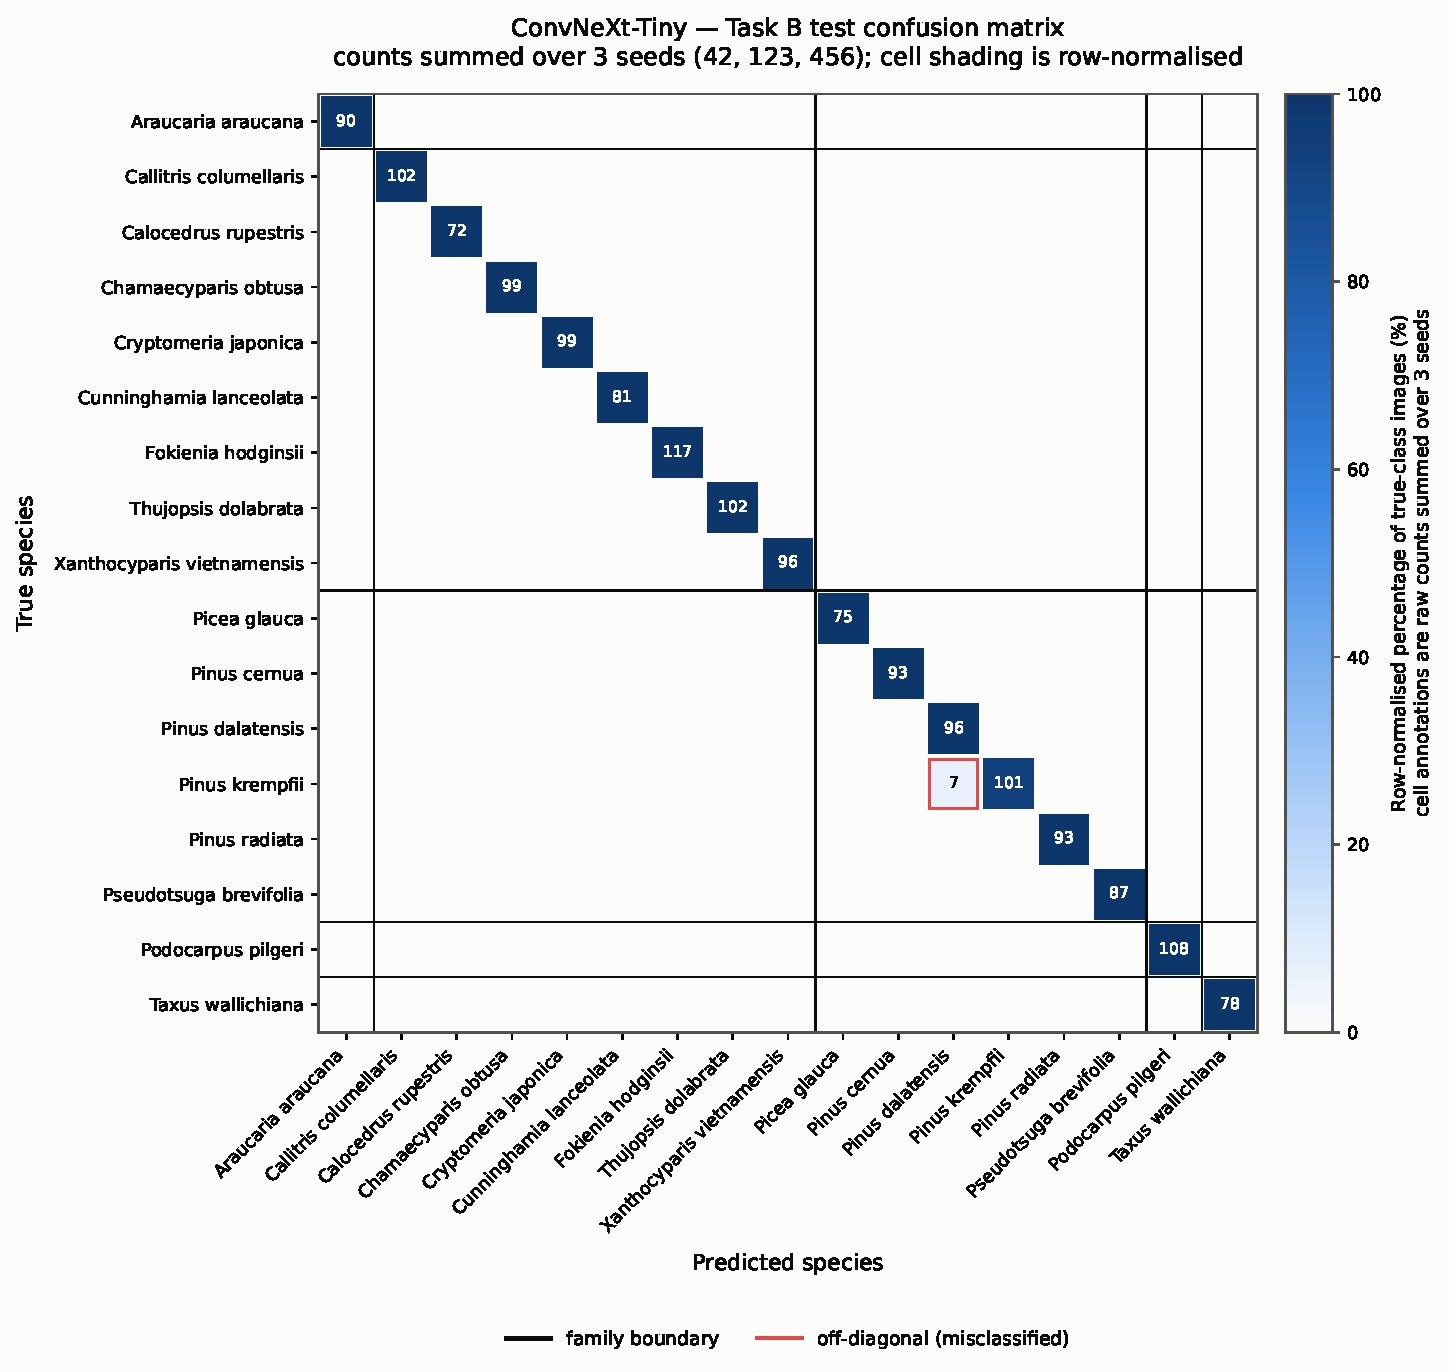
\includegraphics[width=\columnwidth]{artifact/person3/confusion/fig_confusion.pdf}
\caption{Confusion matrix for ConvNeXt-Tiny on the Task~B test set. Counts are
summed element-wise over the three main seeds (42, 123, 456), giving
$532\times3 = 1{,}596$ predictions; each seed contributes equally. Cell shading
is the row-normalised percentage of images of the true class, with the row
total of the summed counts as denominator; the annotation in each cell is the
raw summed count. Species are ordered by family and black rules mark family
boundaries. Off-diagonal cells are outlined in red. ConvNeXt-Tiny was selected
by a criterion fixed in advance --- highest mean macro-F1 over the three seeds
(Table~\ref{tab:task_b}) --- not by inspecting this matrix. The three per-seed
matrices are published alongside the aggregate so that the summation can be
checked.}
\label{fig:confusion}
\end{figure}
